\chapter{Генерация и транспорт убегающих электронов в плазме токамаков, а так же использование сцинтиляционных детекторов для их диагностики}\label{ch:ch1}

\section{Механизмы генерации убегающих электронов}\label{sec:ch1/sec1}

В плазме токамаков имеют место несколько механизмов генерации убегающих электронов. Это:

\begin{itemize}
  \item <<Традиционный>> механизм генерации убегающих электронов в электрическом поле;
  \item Лавинный механизм, при котором первичные убегающие электроны при взаимодействии с электронами основной плазмы перевозят их в режим убегания;
  \item Прочие механизмы, такие как генерация убегающих электронов при распаде трития или при комптоновском рассеянии гамма излучения.
\end{itemize}

Рассмотрим ниже эти механизмы подробнее.

\subsection{Убегание электронов в сильных электрических полях в плазме}

Эффект убегания был предсказан в 1925 году \cite{Wilson1925} и развит в \cite{Dreicer1959}. Пусть в сильноионизованной плазме имеется электрическое поле $E$. Тогда для перехода в режим непрерывного ускорения сила, действующая на электрон со стороны электрического поля, должна превышать силу трения, вызванную кулоновскими столкновениями в плазме:

\begin{equation}
  \label{eq:runawayEq}
  e E >  m_e v_e \nu_{ei}(v_e)
\end{equation}
где $e$ и $m_e$ --- заряд и масса электрона, $\nu_{e}$ --- частота столкновений электрона, $v$ --- скорость электрона \cite{Wesson2004}. Частота кулоновских электрон-ионных столкновений зависит от скорости. Для случая, когда $v \gg \sqrt{ 2 T_e / m_e }$, где $T_e$ --- средняя температура электронов, частота электронных столкновений может быть представлена как 
\begin{equation*}
  \nu_{e}(v) = \frac{ 3 e^4 n \Lambda }{ 4 \pi \epsilon_0^2 m_e^2 v^3 }
\end{equation*} 
где $\Lambda$ --- кулоновский логарифм, $n$ --- концентрация плазмы \cite{Wesson2004}. Графики зависимости силы, действующей на электрон со стороны электрического поля, и силы трения, показаны на рисунке~\ref{fig:runawayForces}.

\begin{figure}[ht]
  \centerfloat{ 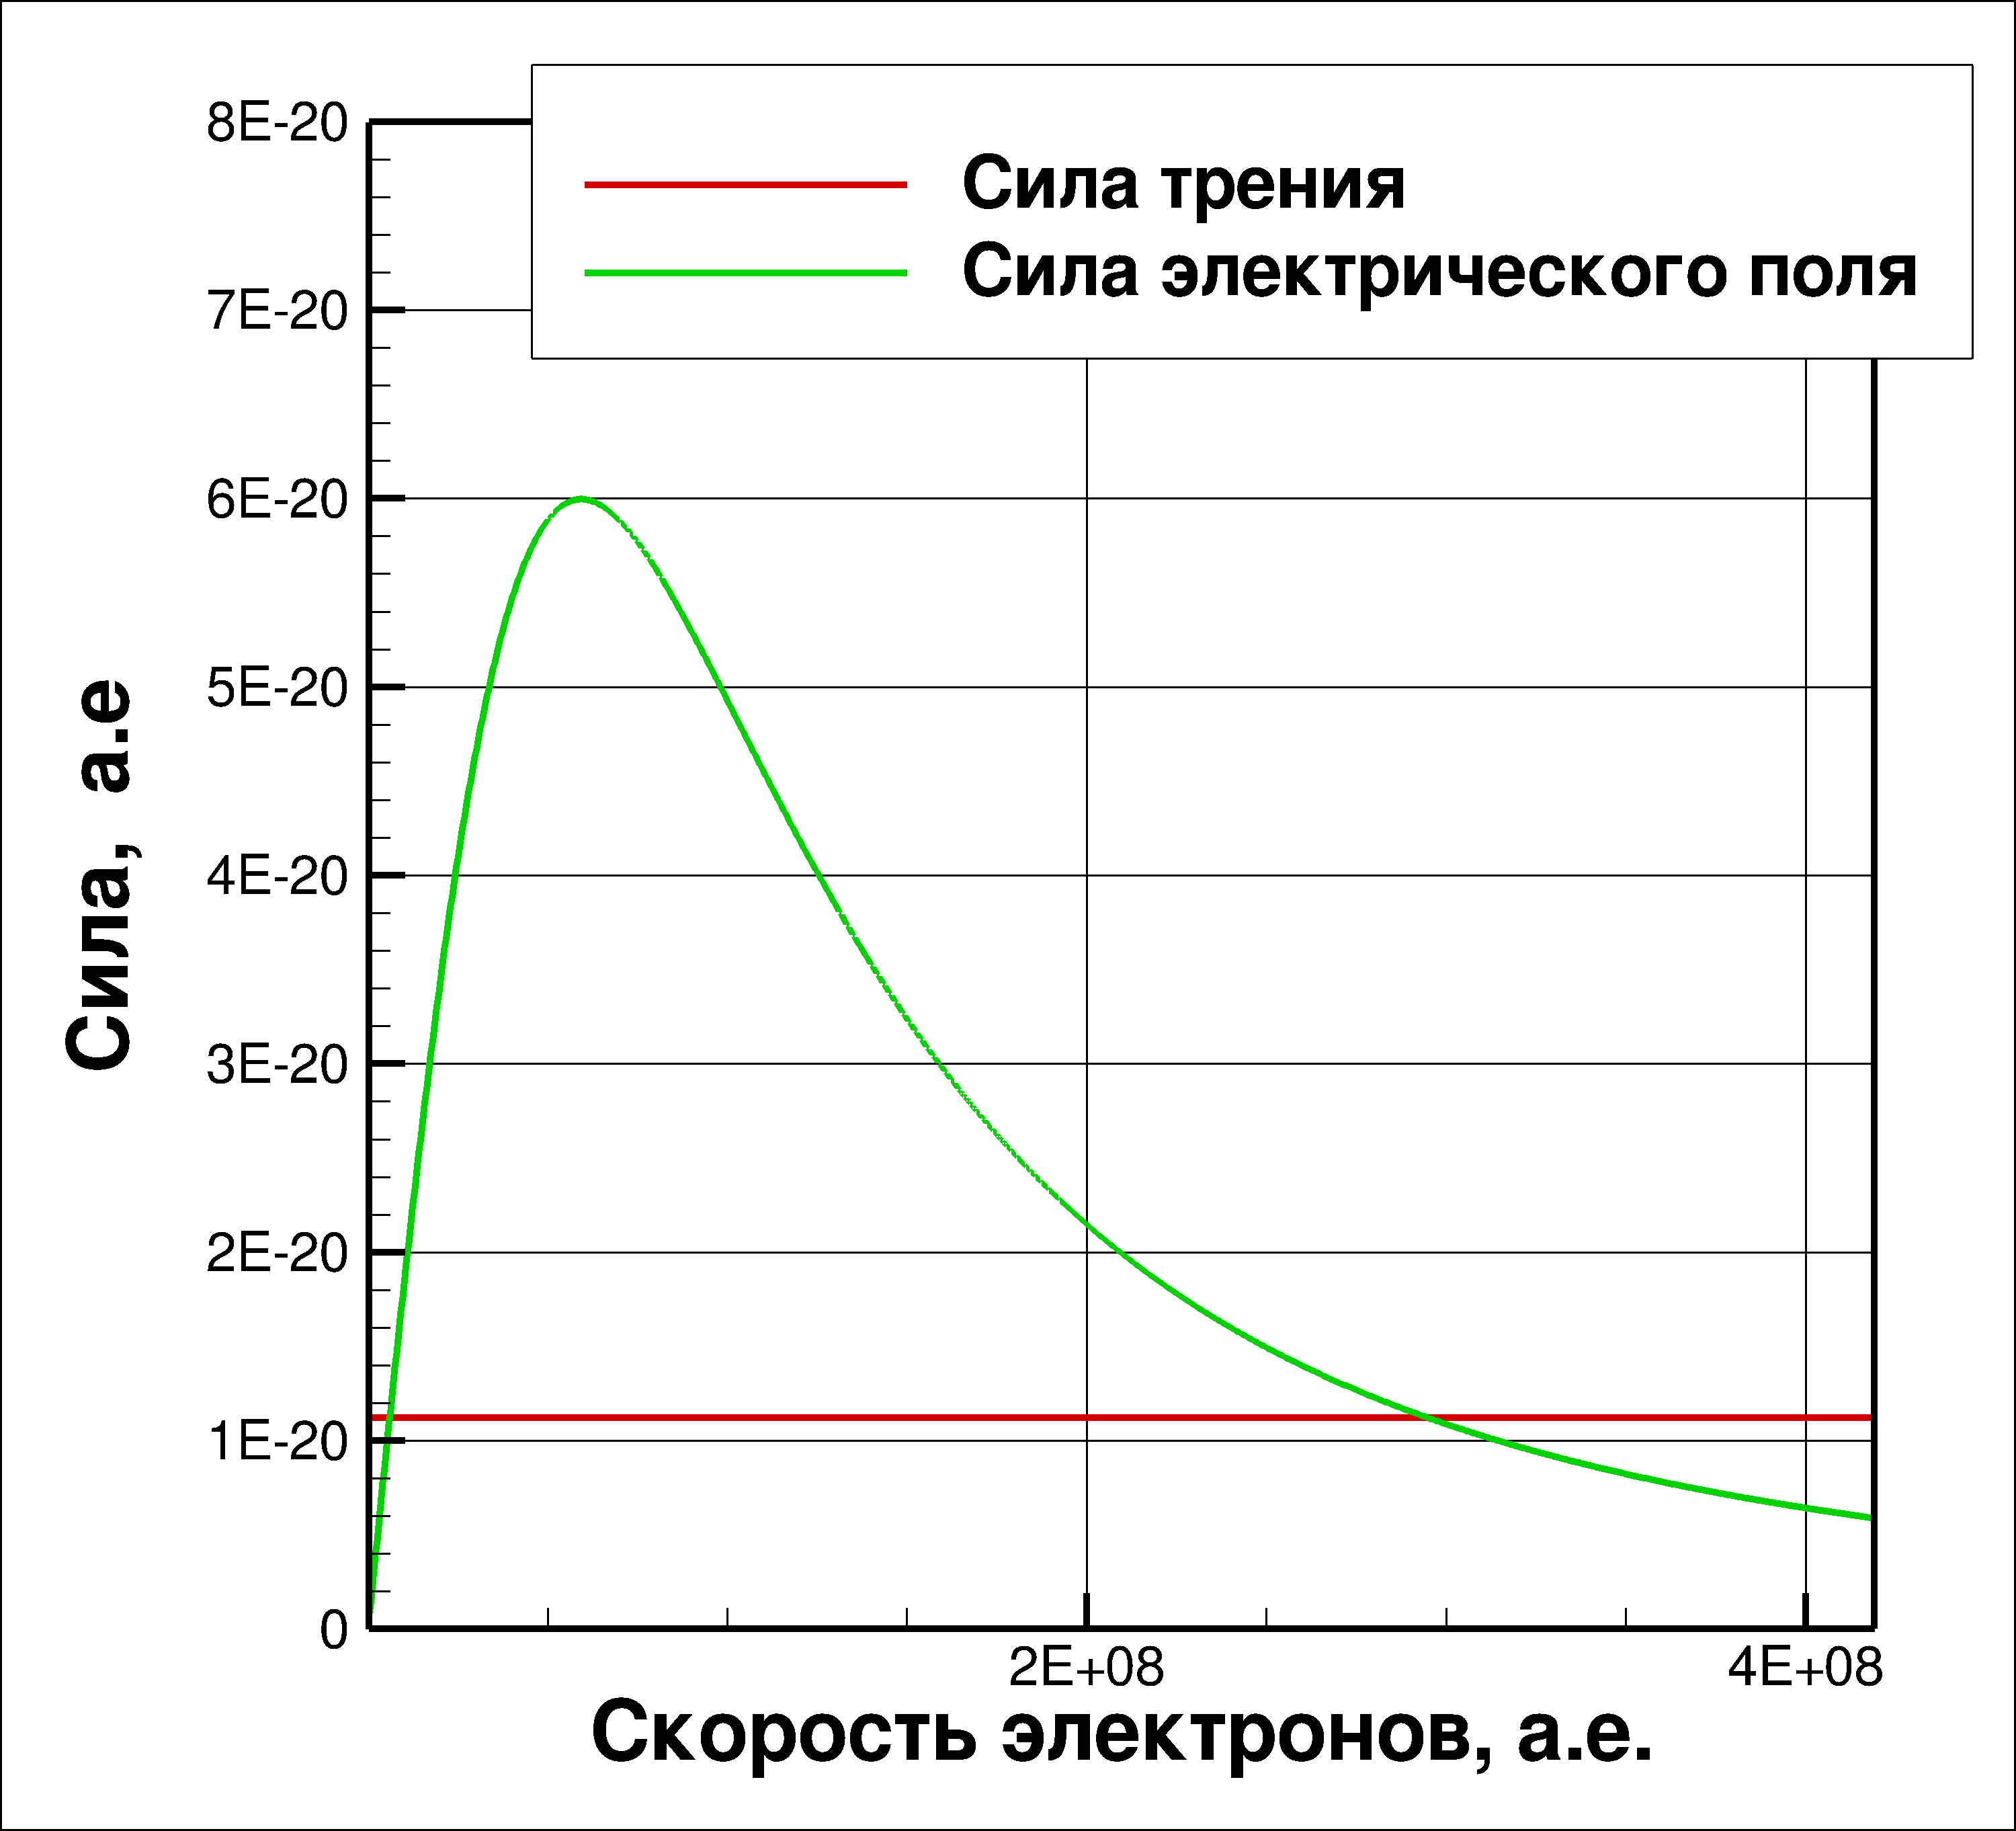
\includegraphics[width=0.60\linewidth]{runawayForces} }
  \caption{ Зависимотсть силы, действующей на электрон со стороны электрического поля и силы трения, которая вычислена по формуле $ C \cdot v/( v^2 + v_{Te}^2 )^{3/2} $~\cite{Golant1977}.}
  \label{fig:runawayForces}
\end{figure}

Можно заметить, что существует некая критическая скорость, начиная с которой неравенство \ref{eq:runawayEq} оказывается истинным. Эта критическая скорость равна
\begin{equation}
  \label{eq:critVelocity}
  v_c = \sqrt{ \frac{ 3 e^3 n \Lambda }{ 4 \pi \epsilon_0^2 m_e E } }
\end{equation}
Если каким-то образом образуется электрон со скоростью, больше критической скорости $v_c$, то он переходит в режим неограниченного ускорения. Такие электроны называются <<убегающими>> \cite{Golant1977}.

Можно рассчитать величину электрического поля, при котором в режим убегания переходят электроны с тепловой скоростью. Это поле оказывается равным 
\begin{equation*}
  E_D = \frac{ n e^3 \Lambda }{ 4 \pi \epsilon_0^2 m_e v_{Te}^2 }
\end{equation*}
и называется полем Дрейсера \cite{Dreicer1959,Golant1977,Wesson2004}. 

Когда электрическое поле достаточно мало, критическая скорость, рассчитанная по уравнению \ref{eq:critVelocity}, приближается к скорости света $c$. Для релятивистских электронов время замедления почти постоянно и существенного уменьшения силы трения с увеличением их энергии уже не происходит. Соответственно, для электрических полей, таких что
\begin{equation*}
  E < E_c = \frac{ n e^3 \Lambda }{ 4 \pi \epsilon_0^2 m_e c^2 }
\end{equation*}
генерации убегающих электронов не происходит ни при каких обстоятельствах \cite{Wesson2004}.

На большем временном масштабе скорость убегания электронов определяется столкновительной диффузией в пространстве скоростей. По мере убегания более быстрых электронов они замещаются электронами, диффундирующими через хвост максвелловского распределения скоростей. Подробные расчеты дают следующую результирующую скорость убегания на единицу объема \cite{Wesson2004}: 

\begin{equation*}
  S_{re} = \frac{2}{ \sqrt{\pi} } n \nu_{e}(v_{Te}) \left( \frac{E}{E_D} \right)^{1/2} \exp\left( -\frac{E_D}{4 E} - \left( \frac{2 E_D }{E} \right)^{1/2} \right)
\end{equation*}

\subsection{Лавинный эффект размножения убегающих электронов}

При кулоновских столкновениях между <<быстрыми>> убегающими электронами и <<медленными>> электронами основной плазмы первые могут передавать вторым часть своей энергией, переводя их в режим убегания \cite{Sokolov1979}. Очевидно, для работы этого процесса требуется, чтобы время жизни убегающего электрона было больше времени между кулоновскими столкновениями. Темп генерации оказывается пропорциональным числу уже существующих в плазме убегающих электронов \cite{Rozansky2012}.  Хотя на пробные частицы в плазме в основном влияют столкновения с большими прицельными параметрами и малым переданным импульсом, в этом процессе большее значение имеет меньшее число близких столкновений, передающих больший импульс. Соответствующие близкие столкновения в этом случае --- это те, которые поднимают медленный электрон выше критической скорости для убегания. 

Импульс, передаваемый медленному электрону быстрым электроном, в основном перпендикулярен скорости $v_f$ быстрого электрона и определяется выражением
\begin{equation*}
  m_e \Delta v \approx 2 m_e v_f \frac{r_0}{r}
\end{equation*}
где $r$ --- прицельный параметр, а $r_0 = e^2 / 4 \pi \epsilon_0 m_e v_f^2$ --- значение прицельного параметра для рассеяния на 90$^\circ$ \cite{Wesson2004}. 

Чтобы столкновение перенесло электрон в область убегания, $\Delta v$ должна быть больше критической скорости, определяемой уравнением \ref{eq:critVelocity}. С учётом этого требования, можно написать сечение для рождения убегающего электрона:
\begin{equation*}
  \sigma(v_f) = \frac{ e E }{ 3 n m_e v_f^2 \Lambda }
\end{equation*}

Считая убегающие электроны релятивистскими, можно положить что $v_f = c$. Тогда скорость рождения новых убегающих электронов оказывается равна следующей величине \cite{Rozansky2012}:
\begin{equation}
  \label{eq:avalanch}
  \frac{ d n_r }{ d t } = n_r \nu_e(c) \left( \frac{E}{E_c} - 1 \right) / \left( 2 \Lambda \right)
\end{equation}

Множитель $E/E_c - 1 $ в формуле \ref{eq:avalanch} показывает, что лавинный механизм генерации убегающих электронов имеет пороговый характер.

Подробно теория генерации убегающих электронов изложена в \cite{Rosenbluth1997}. Лавинный механизм генерации убегающих электронов неоднократно наблюдался в экспериментах; впервые оно было экспериментально обнаружено на токамаке TEXTOR, вероятно имеет место во время срывов на токамаках TFTR, Tore Supra, JT-60U и JET \cite{Gill2002,Helander2002}, было зарегистрировано на токамаке TCABR \cite{Galvao2001}. Анализ распределения по энергии убегающих электронов позволяет предположить, что лавинный механизм может быть доминирующим при генерации убегающих электронов во время срывов, а в срывах JET кажется трудным объяснить ток, переносимый убегающими электронами, не прибегая к этому механизму \cite{Helander2002}.

\subsection{Прочие механизмы генерации убегающих электронов}

Прочие механизмы генерации убегающих электронов носят скорее экзотический характер и не являются существенными на современных установках, однако могут оказывать влияние на более крупных токамаках будущего. Эти механизмы могут служить источником первичных убегающих электронов, которые могут потом размножаться по лавинному механизму за счёт кулоновских столкновений.

При радиоактивном распаде трития, который будет являться одним из компонентов топливной смеси промышленных термоядерных установок, образуется электрон \cite{Burrows1990}:

\begin{equation*}
  T \rightarrow {}^3_2 He + e^{-} + \bar{ \nu_e }
\end{equation*}

Период полураспада трития составляет $ \tau_T = 4500 $ дней, максимальная энергия рождённых в ходе распада электронов равна $ E_{max} = 18.6$~кэВ \cite{MartinSolis2017}. Число убегающих электронов, рождённых за счёт подобного механизма, составляет

\begin{equation*}
  \left( \frac{ d n_{re} }{ d t } \right) \approx \ln(2) \frac{ n_T }{ \tau_T } F_{\beta}(\varepsilon_c)
\end{equation*}

где $\varepsilon_c = m_e v_c^2 / 2$, а 

\begin{equation*}
  F_{\beta}(\varepsilon_c) = \int\limits_{\varepsilon_c}^{ \varepsilon_{max} } f_{\beta}(\varepsilon) d\varepsilon 
\end{equation*}

Тут $ f_{\beta}(\varepsilon) $ --- функция распределения рождаемых в ходе распада электронов от энергии, нормированная на единицу \cite{MartinSolis2017}. Очевидно, что если скорость рождённых в ходе распада электронов меньше, чем скорость, необходимая для перехода в режим убегания, то данный механизм генерации убегающих электронов не функционирует.

В токамаке ИТЭР происходит активация стенок за счёт нейтронов, рождённых в ходе термоядерной DT реакции. Это приводит к тому, что конструкции токамака начинают генерировать гамма излучение. Гамма кванты могут рассеиваться на электронах плазмы, передавая им свою энергию и тем самым потенциально переводя их в режим убегания. Количество создаваемых таким механизмом электронов оказывается равным 

\begin{equation*}
  \left( \frac{ d n_{re} }{ d t } \right) \approx n_e \int \Gamma_{\gamma}(E_{\gamma}) \sigma(E_{\gamma}) d E_{\gamma} 
\end{equation*}

где $\Gamma_{\gamma}(E_{\gamma})$ --- поток гамма квантов с энергией $E_{\gamma}$, $\sigma(E_{\gamma})$ --- сечение рассеяния \cite{MartinSolis2017}.

Графики зависимости скорости генерации убегающих электронов от величины $\varepsilon_c$ для обоих описанных механизмов показан на рисунке~\ref{fig:solisGeneration}.

\begin{figure}[ht]
    \begin{minipage}[b][][b]{0.49\linewidth}\centering
        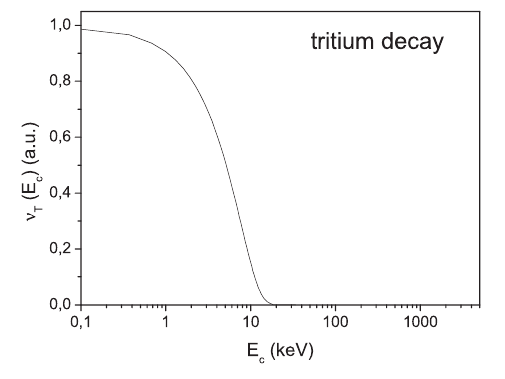
\includegraphics[width=0.95\linewidth]{solisRunawayRenerationTritium} \\ а)
    \end{minipage}
    \hfill
    \begin{minipage}[b][][b]{0.49\linewidth}\centering
        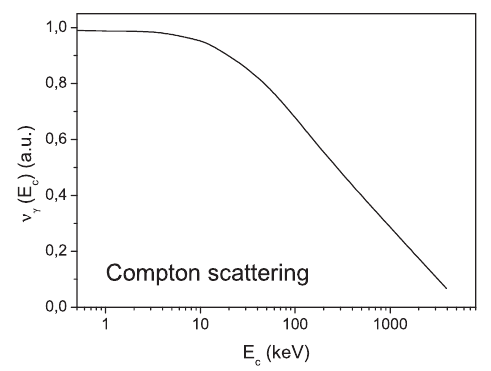
\includegraphics[width=0.95\linewidth]{solisRunawayRenerationCompton} \\ б)
    \end{minipage}
    \caption{ Зависимость скорости генерации убегающих электронов для механизма генерации из электронов, рождённых в ходе радиоактивного распада трития (а) и для механизма генерации за счёт комптоновского рассеяния (б). По вертикальной оси отложена величина $\nu \equiv (1/n_e) \cdot ( dn_r / dt ) $, нормированная на 1 при $\varepsilon_c = 0$; по горизонтальной --- критическая энергия, равная $v_c^2 m_e / 2 $ \cite{MartinSolis2017}. }
    \label{fig:solisGeneration}
\end{figure}



\section{Механизмы ограничения энергии убегающих электронов}

На реальных установках существует ряд механизмов, которые ограничивают максимальную энергию убегающих электронов: 


\section{Методы диагностики убегающих электронов}\label{sec:ch1/sec2}

МОИ ССЫЛКИ: \cite{Khilkevitch2020} \cite{Reux2015}

\FloatBarrier
